\section{Modélisation UML}

En vu dêtre claire et concis sur ce que fournira notre plateforme, il s'est avéré necessaire, une fois la modélisation mathématique terminée, de s'interesser à une modélisation orientée objet en UML. C'est ainsi que pour un début, nous avons conçu les diagrammes d'analyse statique qui suivent:

\subsection{Diagramme de contexte}

\begin{figure}[h]
    \centering
    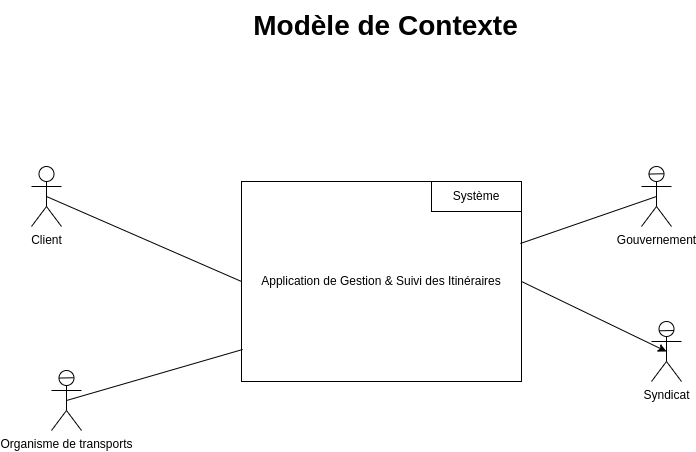
\includegraphics[width=0.8\linewidth]{Images/Diagramme_Contexte.png}
    % \caption{}
    % \label{fig:repartition_trafic}
\end{figure}

Ce diagramme nous permet de représenter notre système dans son environnement, d'avoir une vue externe, globale de ses interactions avec différents types d'acteurs.
Au vu de ce diagramme, on distingue:

\begin{itemize}
    \item \textbf{Système: } Il s'agit de notre application de gestion itinéraires, représenté comme une boite noire, dont le contenu se spécifiera avec les diagrammes qui suivront
    \item \textbf{Acteurs principaux:} Il s'agit des acteurs pour qui est dédié le système. On distingue ainsi
          \begin{itemize}
              \item Le Client: Il s'agit de celui qui vient sur l'application pour avoir le ou les meilleurs itineraire(s) pour se déplacer d'un point A à un point B. Dans le cadre du projet entier, il s'agira d'un conducteur tout court.
              \item Les Organismes de Transport: On voit ici d'éventuelles agences de transports qui pourront faire appel à nos services pour optimiser les déplacements de leurs véhicules
          \end{itemize}
    \item \textbf{Acteurs secondaires:} Ce sont les acteurs qui pourront échanger des informations avec le système, pour son bon fonctionnement. On y retrouve
          \begin{itemize}
              \item Le Gouvernement: Ce sera bien sûr, le régulateur des activités; il pourra même nous fournir des données en matière de mobilité dans un zone spécifique, en vue de l'optimisation des itinéraires.
              \item Syndicat: On parle ici du syndicat des transporteur, qui sera également d'une aide précieuse en vue d'assurer la conformité des conducteurs utilisant la plateforme.
          \end{itemize}
\end{itemize}

\subsection{Diagramme de Package}

\begin{figure}[h]
    \centering
    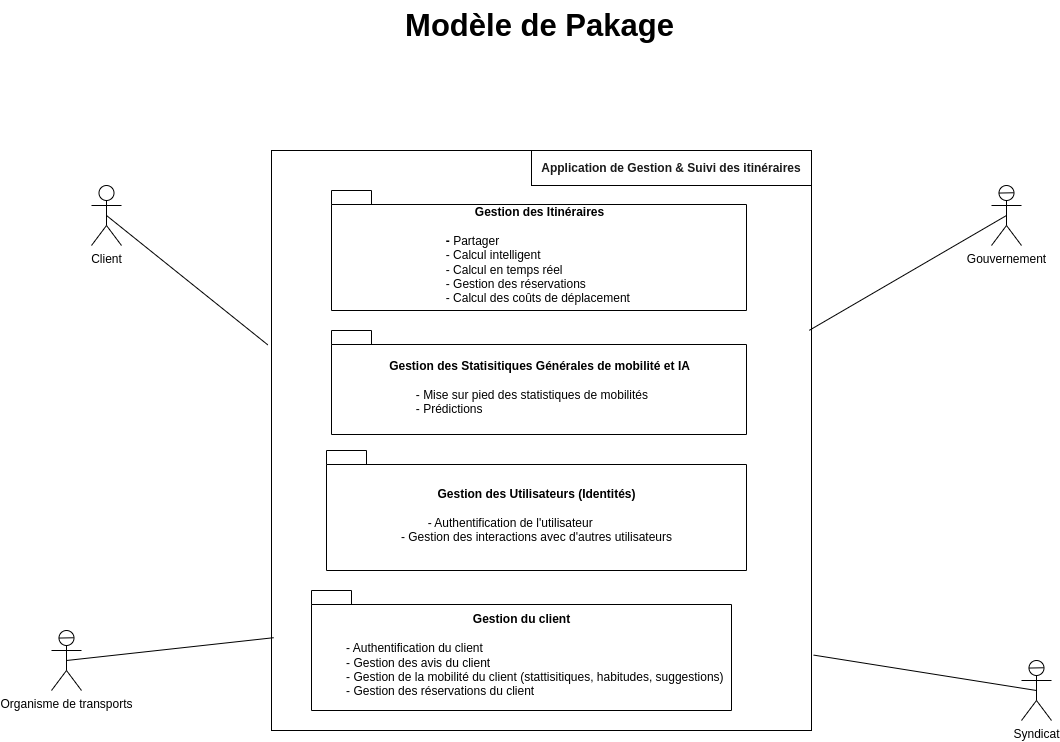
\includegraphics[width=0.8\linewidth]{Images/Diagramme_Package.png}
    % \caption{}
    % \label{fig:repartition_trafic}
\end{figure}

Ce diagramme ci nous permet de voir un peu plus clair dans la boite noire qu'est le système. Comme on peut remarquer sur l'image en amont, on y retrouve:

\begin{itemize}
    \item textbf{Le package de gestion des itinéraires: } C'est la package central, qui va nous permettre de définir modéliser la carte, ses lieux et ses routes, comme expliqués dans le modèle mathématique en amont. On y retrouvera aussi des méthodes pour effectivement calculer les meilleurs itineraires suivant différents filtres, pour évaluer les coûts de déplacements sur ces itinéraires, et même une fonctionnalité pour partager un itineraire.
    \item textbf{Le package de Gestion des Statistiques Générales de mobilité \& IA}: c'est un package ultérieur, qui nous permettra d'ajouter l'IA pour proposer des itinéraires qui tiendront aussi comptes des expériences passées.
    \item textbf{Le package de Gestion des identités:} C'est un package qui nous permettra de stocker les informations de connexion de nos utilisateurs, et qui permettra éventuellement des communications et interactions entre ces derniers. Mais dans il ne sera pas géré dans le cadre de ce projet vu qu'il y'a un autre module du plus grand projet de "Gestion des voyages", dédié à cela.
    \item textbf{Le package de Gestion du Client}: C'est ici qu'on enregistrera tout ce dont on a besoin pour un client qui utilise la plateforme; et c'est également ici, on gérera son interaction avec la plateforme.
\end{itemize}

\subsection{Diagramme de Classe}

\begin{figure}[h]
    \centering
    \includegraphics[width=0.8\linewidth]{Images/Diagramme_Classe.png}
    % \caption{}
    % \label{fig:repartition_trafic}
\end{figure}

Ce diagramme comme on peut le voir nous permet de préciser les classes de notre projet, et leurs relations avec les autres classes.

On a d'un coté les classes liées à la gestion du Client, et de l'autre celles liées à la gestion des itineraires. On peut voir qu'un client à un un WeightEvaluation, on l'on règlera ses filtres en matières de mobilité

\subsection{Diagramme de Deploiement}

\begin{figure}[h]
    \centering
    \includegraphics[width=0.8\linewidth]{Images/Diagramme_Deploiement..png}
    % \caption{}
    % \label{fig:repartition_trafic}
\end{figure}

On arrive à la phase de déploiement où l'on voit de manière synthétique le contenu du système et comment il interagit avec les clients à gauche et avec d'autres services internes, voir d'autres plateformes, via l'API interne, juste en bas. Plus loin on voit que le système communiquera avec l'API d'OpenStreeMap, pour la localisation GPS et l'accès au carte en temps réel.



